% !TEX root = ../00_thesis.tex

%-------------------------------------------------------------------------------
\section{Performance Evaluation}
\label{sec:drp_evaluation}
%-------------------------------------------------------------------------------

After detailing the design~(\cref{sec:designDetailed}) and implementation~(\cref{sec:drp_implementation}) of \DRP, we now evaluate the performance of the system. We consider three different performance aspects.

% However, \DRP provides hard guarantees based on a worst-case analysis, which is pessimistic by design. Thus, we investigate in this section the actual performance that \DRP can achieve.
\begin{itemize}
	\item
	First, we derive the theoretical optimal performances achievable by \DRP, based on the system model~(\cref{subsec:perf_model}).

	\item
	Then, we first use simulation to demonstrate the tightness of the worst-case analysis underlying \DRP's design: we show that end-to-end message latency reaches up to 97\% of the analytic bounds~(\cref{subsec:simulation}).

\pagebreak

	\item
	Finally, we showcase that our \DRP implementation performs as expected: all messages successfully transmitted through the wireless network do meet their end-to-end deadline. Furthermore, we illustrate that on a ``real'' network, messages typically experience latency much shorter than their end-to-end deadline~(\cref{subsec:flocklab}).
\end{itemize}


\begin{remark}
	The \triscale framework, introduced in \cref{ch:triscale}, would be beneficial for the design and analysis of \DRP's performance evaluation.
	However, the evaluation described below is anterior to the work we have done on \triscale, and thus does not use the framework.
\end{remark}


%-------------------------------------------------------------------------------
\subsection{Performance Model}
\label{subsec:perf_model}

The admission tests for \ap and \cp (which ensure that all contracts are satisfied after the admission of a new flow) critically depend on global parameters: the duration of a round \rlength and the deadline ratio $r$.

In this section, we analyze the influence of these parameters on the achievable performance of \DRP in terms of responsiveness (\ie the minimal admissible end-to-end deadline) and bandwidth.

\afterpage{
\begin{figure}
	\centering
	\href{\drpfig{Figure-10}}{%
	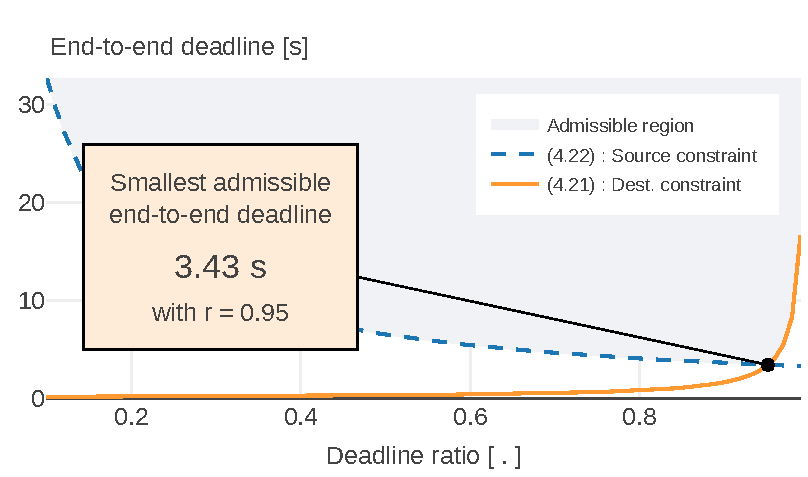
\includegraphics[scale=1]{min_e2edeadline}}
	\caption{The smallest admissible end-to-end deadline for $C_{net} = 1\s$ and $\tfdmin = 0.1\s$ is $\D_{min} = 3.43$\s.
	\capt{%
		Equations \eqref{eq:Dmin_destination_constraint} and \eqref{eq:Dmin_source_constraint} each define a feasible region for $(r,\deadlineany)$ tuples. The intersection defines the admissible region.}
	}
	\label{fig:min_latency}
\end{figure}}

%-------------------------------------------------------------------------------
\fakepar{Responsiveness: Minimal Admissible End-to-end Deadline}
Let us assume that the duration of communication rounds \rlength is given.
\DRP handles messages between application interfaces (\ie the \APs) and constrains the destination \apdst to flush \bolt (at least) every $T_f^d$. Naturally, there exists a lower bound on the admissible $T_f^d$; let us refer to this bound as \tfdmin.
Given these parameters, we are interested in the minimal admissible end-to-end deadline $\D_{min}$, or in other words, the maximal responsiveness of the protocol.

From the previous remark on $T_f^d$ and eq.  \eqref{eq:design_delay_destination} it follows
\begin{align}
\notag
	\tfdmin & \; \leq \; T_f^d \leq \left( (1-r)*\deadlineany - \delta_g^{const} \right)\\
\label{eq:Dmin_destination_constraint}
\Rightarrow \quad
	 \D & \; \geq \; \frac{\tfdmin +  \delta_g^{const}}{(1-r)}
%
\intertext{From \eqref{eq:ndeadline_constraint_latency} we also have}
%
\notag
 T + D + \overline{J}
	& \; \leq  \; r * \deadlineany - \delta_f^{const} \\
\notag
\Rightarrow \quad
	 \D & \; \geq \; \frac{T + D + \overline{J} + \delta_f^{const} }{r}
%
\intertext{%
We look for the minimal expression of the right-hand side term.
\eqref{eq:ndeadline_constraint_period} : $T_{net}^{min} \leq D_i \leq T_i$\; yields $T_{min} = D_{min} = T^{min}_{net}$.
Moreover, combining \eqref{eq:design_flush_period_source} and \eqref{eq:design_round_period} entails $T^{min}_{net} = T^s_f  = C_{net} + C_{CP}$. Hence $T_{min}$ is fixed given $C_{net}$.
Finally, in the best case, there is no (or small) jitter (\ie $\overline{J}=0$), and we obtain}
\label{eq:Dmin_source_constraint}
\Rightarrow \quad
	 \D & \; \geq \;	\frac{2T_{min} + \delta_f^{const}}{r}
\end{align}
\eqref{eq:Dmin_destination_constraint} and \eqref{eq:Dmin_source_constraint} define two lower bounds on the minimal admissible end-to-end deadline $\D_{min}$ induced by the contracts. Combining them, it follows that
\begin{align}
\notag &\D_{min} \;=\; \min_r
	\left(
	\frac{\tfdmin +  \delta_g^{const}}{(1-r)}
	\, , \,
	\frac{2T_{min} + \delta_f^{const}}{r}
	\right)
%
\intertext{The minimal value $\deadline{min}$ is reached for}
r_{opt} \;&=\; (2T_{min} + \delta_f^{const} )/(\tfdmin + \delta_g^{const} + 2T_{min} + \delta_f^{const})
%
\intertext{and it yields}
%
	&\D_{min} \;=\; \tfdmin + 2T_{min} + \delta_f^{const} + \delta_g^{const}
\end{align}

Using the parameters in \cref{table:simulation_parameters} from real-world prototypes, if $\rlength = 1$\s  and $\tfdmin = 0.1$\s, the minimal end-to-end deadline that can be supported is $\D_{min} = 3.43\s$, with $r = r_{opt} = 0.95$, and the minimum message interval $T = T_{min} = 1.074\s$. This case is illustrated in \cref{fig:min_latency}.
\TODO{rewrite as a table}


\begin{table}
\centering
\caption{Simulation parameters.
\capt{
	The \bolt API execution times are formally proven bounds for the given hardware~\cite{sutton2015Bolt}.
	The number of slots per round \nslotsmax is defined as the number of slots that ``fit'' into a round of length \rlength given the packet size.
	}}
{\smaller
\begin{tabular}{@{}c@{\qquad}l@{\qquad}c@{\qquad}l@{}}
\toprule
	&\textbf{Parameter}
	& \textbf{Symbol}
	& \textbf{Value} \\
\midrule
&WCET of \opwrite
	& $C_w$
	& $116 \us$\\
\bolt &WCET of \opread
	& $C_r$
	& $112 \us$\\
&WCET of \opflush
	& $C_f$
	& $684 \ms$\\
\midrule
&Round length
	&$C_{net}$
	& $1 \s$ \\
\blink &Packet size
	& $L$
	& $32$\bytes \\
&Max number of slots in one round
	&\nslotsmax
	& $46$ \\
\midrule
&Number of nodes
	& .
	& $20$ \\
\DRP &Deadline ratio
	& $r$
	& $0.5$ \\
&Flushing interval of $\cp$
	& $T_f^s$
	& $1.074 \s$ \\
\bottomrule
\end{tabular}}
\label{table:simulation_parameters}
\end{table}

%-------------------------------------------------------------------------------
\fakepar{Bandwidth: Maximal Duration of Communication Rounds}
Conversely, let us now assume that the minimal end-to-end deadline to be supported is given by $\D$, and consider the same assumption on $T_f^d$. The maximal bandwidth achievable by \blink is $\nslotsmax/T_{net}^{min}$ \pkts/\s. The round length $C_{net}$ is a linear function of the number of packets per round \nslotsmax (\ie a constant time per packet plus some overhead), and \linebreak
\eqref{eq:design_round_period} : $T_{net}^{min} = C_{net} + C_{CP}$. Hence, the maximal bandwidth actually grows with $C_{net}$. Thus, we now investigate the maximal admissible duration of communication rounds $C_{net}$ that yields the maximum available network bandwidth.

From \eqref{eq:ndeadline_constraint_latency} we have
$T + D + \overline{J}\;
	\leq  \; r * \deadlineany - \delta_f^{const}$, and, \linebreak
as previously, $T_{net}^{min} = C_{net} + C_{CP} \leq D \leq T$.
We get
\begin{align}
\label{eq:C_net_f(r)}
& C_{net}
		\;\leq\;
		 \frac{1}{2}
		 	(r * \deadlineany - \delta_f^{const}) - C_{CP}
%
\end{align}
From \eqref{eq:Dmin_destination_constraint}, given \deadlineany and \tfdmin, the maximal admissible value for $r$ is $\displaystyle r_{max} = 1 - ({\tfdmin + \delta^{const}_g}) / \deadlineany$ , and finally
\begin{align}
\label{eq:C_net_upperbound}
	& C_{net}
		\,\leq\,
		 \frac{1}{2}
		 	\left(
		 	\deadlineany - \delta_f^{const}- \delta_g^{const} - \tfdmin
		 	\right)
		 - C_{CP}
\end{align}

Using the parameters from \cref{table:simulation_parameters}, if we need to satisfy end-to-end deadlines of $\deadlineany = 10$\s and $\tfdmin = 3$\s, the maximal round length that can be supported is $\rlength = 2.82$\s, with $r = r_{max} = 0.69$, and the minimum message interval $T = C_{net} + C_{CP} = 2.89\s$. That upper-bound also yields the maximal achievable network bandwidth.
\TODO{rewrite as a table}

%-------------------------------------------------------------------------------
\fakepar{Effect of Deadline Ratio on System Performance}

We presented earlier that given $C_{net}$ and \tfdmin, there is an optimal value for $r$ that minimizes the admissible end-to-end deadline \deadlineany. If one tolerates ``larger'' deadlines, $r$ can be increased to allow for a bigger round length $C_{net}$ (see \eqref{eq:C_net_f(r)}), which increases the maximal network bandwidth.

However, \eqref{eq:design_delay_destination} yields $T_f^d \leq (1-r)*\deadlineany - \delta_g^{const}$. Hence, the bigger $r$ is the smaller $T_f^d$ must be, which may results in more flows rejected by the destination application.
On the contrary, if $r$ is set to its minimal value \linebreak
$\;r_{min} = ({2*T_{min} +  \delta^{const}_g})\, /\, {\deadlineany}$ (obtained from eq. \eqref{eq:Dmin_source_constraint}), it yields $T = \ndeadlineany = T_{min} = 1.074$\s and $\overline{J} = 0$\s. In other words, the maximal admissible jitter (obtained from \eqref{eq:jitter_bar}) is \linebreak
$J < T_f^s + C_r - C_f \approx 0.390$\s.
\TODO{space out a bit.}

How to set the parameters for \DRP depends on the application. For instance, if one consider an acoustic sensing scenario, responsiveness is usually quite critical, and the sensors (\ie the \APs) should spend most of their time on sensing, not being busy with flushing \bolt. Thus, we want to support a rather small $\D_{min}$ while having a strong constraint on \tfdmin. This will come at the cost of a "small" network bandwidth.
